\documentclass[acmsmall,screen]{acmart}
  \citestyle{acmauthoryear}
  
  % \documentclass[acmsmall,10pt]{acmart}\settopmatter{printfolios=true} % ,review
% \citestyle{acmauthoryear}
\usepackage{subcaption}
\usepackage[T1]{fontenc}
\usepackage[utf8]{inputenc}
\usepackage[british]{babel}
\usepackage{xspace, listings, lstcustom, wrapfig, graphicx, enumerate}
\usepackage{paralist}
\usepackage{color, colortbl, relsize}
\usepackage{rotating}
\usepackage{pifont}
\usepackage{multirow}
\usepackage{soul}
\usepackage{tcolorbox}
\usepackage[scaled=.9, light]{zlmtt}
\usepackage{siunitx}
\usepackage{setspace}

   \newcommand{\ttt}{\prg{true}}
\newcommand{\ff}{\prg{false}}
\newcommand{\unkn}{\prg{b???}}
\newcommand{\bv}{\prg{bval}}

\newcommand{\sdparagraph}[1]{{\vspace{.3cm} \noindent \textit{#1}\ }}

\newcommand{\prg}[1]{{\mbox{\tt{#1}}}}

\newcommand{\m}{\prg{m}}
 \newcommand{\f}{\prg{f}}
  \newcommand{\e}{\prg{e}}
 \renewcommand{\c}{\prg{C}}
 \renewcommand{\v}{\prg{v}}
  \newcommand{\x}{\prg{x}}
  \newcommand{\p}{\prg{p}}
   \newcommand{\y}{\prg{y}}
      \newcommand{\uu}{\prg{u}}
  %  \newcommand{\z}{\prg{z}}
  \newcommand{\this}{\prg{this}}
  \newcommand{\caller}{\kw{caller}}
   \newcommand{\nullK}{\prg{null}}
\newcommand{\addr}{\ensuremath{\alpha}}


\newcommand{\fldMap}{\textit{fldMap}}

\newcommand{\forget}[1]{}
\newcommand{\etc}{{\it etc.}}
\newcommand{\eg}{{\it e.g.\,}}
\newcommand{\ie}{{\it i.e.\,}}

% new macros for holistic
\newcommand{\Future}[1] {\ensuremath{{\mathsf{will}}\langle \,#1\,\rangle}}
\newcommand{\Using}[2]{\ensuremath{\langle\, #1\, \mathsf{in}\, #2\, \rangle}}
\newcommand{\External}[1] {\ensuremath{{\mathsf{external}}\langle\,  #1\, \rangle}}
\newcommand{\Internal}[1] {\ensuremath{{\mathsf{internal}}\langle\,  #1\, \rangle}}
\newcommand{\Changes}[1]{\ensuremath{{\mathsf{changes}}\langle\,#1\,\rangle}}
\newcommand{\CanAccessTr}[2]{\ensuremath{\langle\, #1\, \mathsf{access}^*\, #2\, \rangle}}
\newcommand{\CanAccess}[2]{\ensuremath{\langle\, #1\, \mathsf{access}\, #2\, \rangle}}

\newcommand{\Calls}[4]{\ensuremath{\langle\, #1\, \mathsf{calls}\, #3.#2\lp#4\rp\, \rangle}}%(\!({#1})\!)}
\newcommand{\Next}[1] {\ensuremath{{\mathsf{next}}\langle \,#1\,\rangle}}%(\!({#1})\!)}
\newcommand{\PrevId}{\ensuremath{{\mathcal{P}}\textrm{\textit{rev}}}}
\newcommand{\Prev}[1] {\ensuremath{{\mathsf{prev}}\langle \,#1\,\rangle}}%(\!({#1})\!)}
\newcommand{\Past}[1]  {\ensuremath{{\mathsf{was}}\langle \,#1\,\rangle}}

\newcommand{\Name}[2]  {\ensuremath{{\mathsf{name}}\langle \,#1, #2\rangle}}

% old macros for holistic
%\newcommand{\Future}[1] 
%{{{\mathcal W}\!ill}\langle#1\rangle}%{\lozenge\, #1}% {\bullet #1}% {{{\mathcal F}}(#1)} % {{{\mathcal B}}(#1)}
%\newcommand{\Using}[2]{{\mathcal W}ith\langle\ #2,\,#1\ \rangle}
% \newcommand{\External}[1]{{\mathcal E}xternal\langle #1\rangle}
%\newcommand{\Using}[2]{#1\,{\mathcal U}sing\, #2}
%\newcommand{\Using}[2]{#1\,{\mathcal U}sing\, #2} %{{{\mathcal U}}(#1,#2)}
% \newcommand{\Changes}[1]{\ensuremath{\mathcal{C}\textrm{\textit{hange}}\langle#1\rangle}}
%\newcommand{\CanAccessTr}[2]{\ensuremath{\mathcal{A}}\textrm{\textit{ccess}}^*\langle #1,#2\rangle}
%\newcommand{\CanAccess}[2]{\ensuremath{{\mathcal{A}}\textrm{\textit{ccess}}}\langle #1,#2\rangle}%(#1,#2)}
%\newcommand{\Calls}[4]{\ensuremath{{\mathcal{C}}\textrm{\textit{alls}}}\langle #1,#2,#3,#4\rangle}%(\!({#1})\!)}
%\newcommand{\Next}[1]{\ensuremath{{\mathcal{N}}\textrm{\textit{ext}}}\langle #1\rangle}%(\!({#1})\!)}
%\newcommand{\PrevId}{\ensuremath{{\mathcal{P}}\textrm{\textit{rev}}}}
%\newcommand{\Prev}[1]{\ensuremath{{\mathcal{P}}\textrm{\textit{rev}}}\langle #1\rangle}%(\!({#1})\!)}
%\newcommand{\Caller}{\ensuremath{{\mathcal{C}}\textrm{\textit{aller}}}}

%\newcommand{\VisibleLit}{\ensuremath{\mathcal{V}\textrm{\textit{isible}}}}
%\newcommand{\Next}[1]{\ensuremath{{\mathcal{N}}\textrm{\textit{ext}}}\langle #1\rangle}%(\!({#1})\!)}
%\newcommand{\PrevId}{\ensuremath{{\mathcal{P}}\textrm{\textit{rev}}}}
%\newcommand{\Prev}[1]{\ensuremath{{\mathcal{P}}\textrm{\textit{rev}}}\langle #1\rangle}%(\!({#1})\!)}
%\newcommand{\Caller}{\ensuremath{{\mathcal{C}}\textrm{\textit{aller}}}}
% \newcommand{\Past}[1] {{{\mathcal W}\!as}\langle#1\rangle}% {\nabla #1} %{\lozenge\!\!\!\!\-\!\!-\,#1}


\newcommand{\SigmaUsing}[2]{#1\@ #2} %{{{\mathcal U}}(#1,#2)}
%{\lozenge\!\!\!\!\!\circ  #1} % {\lozenge\!\!\!\!\-\!\!- #1} %{\upupsilon #1}  %{\nabla #1} %{\circ #1}%  {{{\mathcal P}}(#1)}
\newcommand{\Initial}[1] {{{\mathcal I}\!nitial}\langle#1\rangle}

\newcommand{\Pol}[1] {{\ensuremath{\prg{Pol}\_{\prg{#1}}}}}

\newcommand{\strongImplies}{\leqq} %{{ \,^\sqsubset\!\!\!_{\sim}\, }}
\newcommand{\weakImplies}{\lessapprox} %{{ \,^\sqsubset\!\!\!_{\sim}\, }}
\newcommand{\frames}{~\kw{frames}~}

\newcommand{\appref}[1]{see App.~\ref{#1}}

\newcommand{\sE}{{\prg{e}}}
\newcommand{\varMap}{{\ensuremath{\beta}}}

\newcommand{\Lang} {\ensuremath{{\mathcal L}{_1}}}
\newcommand{\LangOO} {\ensuremath{{\mathcal L}{_{\tt {oo}}}}\xspace}
\newcommand{\Chainmail} {\ensuremath{{\mathcal C}hainmail}\xspace}

% ------------------------------------------------------------------
%                                             positions, separations
\newcommand{\cf}{{\it c.f.~}}
\newcommand{\HYPHENA}{{\em-- }}
\newcommand{\HYPHENB}{{\em-- }}
\newcommand{\SP}{{\hspace{.1in}}}
\newcommand{\s}{{\hspace{.01in}}}

\newcommand{\obeys}{\,\textbf{\textrm{obeys}}\,}
\newcommand{\StrongDom}{\ensuremath{\mathcal{S}\textrm{\textit{trong}}{\mathcal{D}}\textrm{\textit{om}}}}
\newcommand{\Dom}{\ensuremath{\mathcal{D}}\textrm{\textit{om}}}


\newcommand{\Gives}{\ensuremath{\mathcal{G}\textrm{\textit{ives}}}}
%{\ensuremath{\mathcal{C}\textrm{\textit{an}}{\mathcal{A}}\textrm{\textit{ccess}}}(#1,#2)}
\newcommand{\A}{\ensuremath{A}}
\newcommand{\B}{\ensuremath{B}}
\newcommand{\Arising}[1]{{\mathcal{A}}\textrm{\textit{rising}}(#1)}

 %------------------------ syntax tables

\newcommand{\syntax}[1]{\prg{{\it #1}}}
\newcommand{\BBC}{$::=$} %in syntactic definitions
\newcommand{\SOR}{\ensuremath{\ \mid\ }} % BNF or
\newcommand{\MID}{{\SPsmall ~ \mid ~ \SPsmall }} % in sets


\newcommand{\pre}{\ensuremath{_{{pre}}}}   %kjx no \sc  in math mode
\newcommand{\post}{\ensuremath{_{{post}}}} %kjx no \sc  in math mode
\newcommand{\PRE}{\pre}
\newcommand{\POST}{\post}

 \newcommand{\interp}[2]{{\ensuremath{\lfloor{ {#1}}\rfloor_{#2}}}}
% \newcommand{\interpBL}[1]{{\lceil   {#1}  \rfloor}}

% ------------------------------------------------------------------
%                                              keywords, program text
\newcommand{\kw}[1]{\prg{#1}} % {{\bf{\sf {#1}}}}
\newcommand{\kwN}[1]{{\bf{\sf {#1}}}}
\newcommand{\returnKW}{{\bf{\sf {return}}}}
\newcommand{\newKW}{\mbox{\bf{\sf{new}}}}

\newcommand{\lit}[1]{{\prg {#1}\xspace}}
\newcommand{\com}{\ensuremath{\prg{//}}}


\newcommand{\ass}{\mbox{{\kw {:=}}\,}}
\newcommand{\semi}{\mbox{{\kw {;}}\ }}
\newcommand{\comma}{\mbox{{\kw {,}}\,}}
\newcommand{\lb}{\prg{\mbox{\tt{\bf{\{ }}}}}
\newcommand{\rb}{\prg{\mbox{\tt{\bf{\} }}}}}
\newcommand{\lp}{\prg{\mbox{\tt{\bf{( }}}}}
\newcommand{\rp}{\prg{\mbox{\tt{\bf{) }}}}}
%\newcommand{\thisL}{{\lit {this}}}% no~around it
\newcommand{\nullKW}{{\lit {null}}~}
\newcommand{\true}{{\lit {true}}~}
\newcommand{\false}{{\lit {false}}~}
\newcommand{\return}{{\kw {return}}\s}

 \newcommand{\M}{\prg{\ensuremath{\prg{M}}}}
  \newcommand{\Prog}[1]{\M{#1}}

\newcommand{\mkpair}{\fatsemi}
\newcommand{\subconf}{\ensuremath{\sqsubseteq}}
\newcommand{\restrct}[2]{\ensuremath{#1\!\!\downarrow\!_{#2}}}
\newcommand{\adapt}{\ensuremath{\!\triangleleft\!}}
\newcommand{\link}{\!\circ\!}

\newcommand{\ClassOf}[2] {\ensuremath{{\mathcal C}{\mathit{lass}}(#1)_{#2}}}

% --- assertions and expressions - simple

\newcommand{\SA}{\ensuremath{B}}%{\ensuremath{\prg{B}}}
\newcommand{\SAPrime}{\ensuremath{B'}}

\newcommand{\SE}{\ensuremath{\prg{e}}}
\newcommand{\SEPrime}{\ensuremath{\prg{e}'}}
\newcommand{\SEOne}{\ensuremath{\prg{e}_1}}
\newcommand{\SETwo}{\ensuremath{\prg{e}_2}}




%\newcommand{\Prog}[1]  {{\ensuremath{\prg{M}{{\prg{#1}}}}}}
    % {\prg{P}}

\newcommand{\expandexp}[1]{}

\newcommand{\oo}{object-oriented}
\newcommand{\mExtS}{\ensuremath{\Downarrow}}

% re-classification expression
\newcommand{\cm}[1]{\this{\prg{\ensuremath{\mExtS}}}\prg{#1}}

\newcommand{\refDef}[1]{Definition \ref{{#1}}}

% structuring macros
\newcommand{\EndDefLemma}{\noindent $\bigtriangleup$}

 %-------------------- implies, and, or, iff, etc -----------------
  \newcommand{\AND}{{\SPsmall {\mbox{and}} \SPsmall}}
\newcommand{\WITH}{{\SPsmall {\mbox{with}} \SPsmall}}
 \newcommand{\IFF}{{\SP {\mbox{ if }} \SP}}
\newcommand{\OR}{{\SPsmall {\mbox{or}} \SPsmall}}
%\newcommand{\implies}{{\ensuremath{\longrightarrow}}}
\newcommand{\upd}{{\mapsto}}

\newcommand{\SAF}{\ensuremath{W}} % {\prg{AFs}}






%Macros for inference rules
\newcommand{\inferencerule}[2]{
\begin{array}{l} #1 \\ \hline #2 \end{array}
}


\newcommand{\inferenceruleExact}[4]
{
\begin{array}{l}
{#1}  {\sf #2}
\\ #3  \\ \hline   #4
  \end{array}
}

\newcommand{\inferenceruleN}[3]
{
\begin{array}{l}
%\SP\SP\SP\SP\SP\SP\SP\SP
\SP\SP\SP\SP\SP  {\sf #1}
\\ #2  \\ \hline   #3
  \end{array}
}

\newcommand{\inferenceruleNM}[3]
{
\begin{array}{l}
\SP\SP\SP\SP\SP \SP\SP\SP\SP\SP\SP\SP\SP  {\sf #1}
\\ #2  \\ \hline   #3
  \end{array}
}

\newcommand{\inferenceruleNN}[3]
{
\begin{array}{l}
\SP\SP\SP\SP\SP\SP\SP\SP
\SP\SP\SP\SP\SP\SP\SP\SP
\SP\SP\SP\SP\SP\SP\SP\SP
\SP\SP\SP\SP\SP\SP\SP\SP
\SP\SP\SP\SP\SP\SP\SP\SP
\SP\SP
   {\sf #1}
\\ #2  \\ \hline   #3
  \end{array}
}

%===========================================================================
%  Definition-Lemma-Theorem-Proof
%
% Adaptation of LaTeX's theorem environment; can be used as a command
% (eg just \Lemma not \begin{Lemma}) and no italicisation; also works
% with ptmac; result numbering is uniform within subsections and can be
% suppressed.
%
\newif\ifNumberResults\NumberResultstrue
\def\@@opargbegintheorem#1#2#3{\@@@@begintheorem{\bf\@@thmname{#1}{#2}(#3)}}
\def\@@begintheorem#1#2{\@@@@begintheorem{\bf\@@thmname{#1}{#2}}}
\def\@@@@begintheorem#1{\par\removelastskip\smallskip\noindent{#1}}
\def\@@thmname#1#2{#1\ \ifNumberResults#2\ \fi}

% similarly \Proof or \begin{Proof}...\end{Proof}
% prefer proofs with statements if possible - hence \penalty700
%\let\qedsymbol\S% make it \square or \blacksquare if you like for kb
\let\qedsymbol \Box
\def\qed{\hfill{$\qedsymbol$}}
\def\Proof{\par\removelastskip\smallskip\penalty700\noindent{\bf Proof}\enskip}
\def\endProof{\qed\penalty-700 \smallskip}
\let\endproof\endProof

%   The actual words

\newtheorem{theo}{Theorem}
\newtheorem{definition}[theo]{Definition}
%\newtheorem{example}[theo]{Example}
\newtheorem{mylemma}[theo]{Lemma}
%\newtheorem{conjecture}[theo]{Conjecture}
% \newtheorem{theorem}{Theorem}
% \newtheorem{note}[theo]{Note}
 \newtheorem{observation}[theo]{Observation}


%--------------------------------- the ones that Susan introduced
\newcommand{\SF}{{\prg S}}
\newcommand{\z}{{\prg z}}
\newcommand{\pu}{{\prg u}}
\newcommand{\pb}{{\prg b}}
\newcommand{\acc}{{\prg a}}
\newcommand{\bal}{{\prg{balance}}}
\newcommand{\zs}{{\prg{zs}}}

\newcommand{\Fields}[3]{\ensuremath{{\mathcal F}(}\Prog{#1},\prg{#2},
\prg{#3}\ensuremath{)} }
\newcommand{\FieldIds}[2]{\ensuremath{{\mathcal F}{\it {s}}(\Prog{#1},\prg{#2})}}
\newcommand{\Meths}[3]{\ensuremath{{\mathcal M}(}\Prog{#1},\prg{#2},
\prg{#3}\ensuremath{)} }





\newcommand{\WideFig}[3]
{
\begin{figure*}[t]
\begin{center}
\noindent
\fbox{
\begin{minipage}{4.7 in}
{#1} % the contents
\end{minipage}
}
\caption{#2}
\label{#3}
\end{center}
\end{figure*}
}


\newcommand{\WideFigWhere}[4] % you can specify where it should appear!
{
\begin{figure*}[{#4}]
\begin{center}
\noindent
\fbox{
\begin{minipage}{5. in}
{#1} % the contents
\end{minipage}
}
\caption{#2}
\label{#3}
\end{center}
\end{figure*}
}

\newcommand{\BigWideFigWhere}[4] % you can specify where it should appear!
{
\begin{figure*}[{#4}]
\begin{center}
\noindent
{\normalsize
\hrule
\begin{minipage}{5. in}
{#1} % the contents
\end{minipage}
\hrule
}
\caption{#2}
\label{#3}
\end{center}
\end{figure*}
}

\newcommand{\NotTooWideFigWhere}[4] % you can specify where it should appear!
{
\begin{figure*}[{#4}]
\begin{center}
\noindent
\fbox{
\begin{minipage}{4.3 in}
{#1} % the contents
\end{minipage}
}
\caption{#2}
\label{#3}
\end{center}
\end{figure*}
}


\newcommand{\opsemExprFig}
{\BigWideFigWhere {\opsemExpr} {Execution of expressions\MD}
{opsemTrad} {htbp} }



\newcommand{\mlc}{ }%{\heartsuit}
%\newcommand{\mcl}{ }%{\heartsuit}
\newcommand{\mc}{ }%{\heartsuit}

\newcommand{\BigNotTooWideFigWhere}[4] % you can specify where it should appear!
{
\begin{figure*}[{#4}]
\begin{center}
\noindent
{\normalsize
\hrule
\begin{minipage}{4.3 in}
{#1} % the contents
\end{minipage}
\hrule
}
\caption{#2}
\label{#3}
\end{center}
\end{figure*}
}

 \newcommand{\hlc}[2][yellow]{{%
    \colorlet{foo}{#1}%
    \sethlcolor{foo}\hl{#2}}%\prg{m}''
}

%]})
%}


% \setcopyright{rightsretained}
%\acmPrice{}
%\acmDOI{10.1145/3133896}
%\acmYear{2018}
%\copyrightyear{2018}
%\acmJournal{PACMPL}
%\acmVolume{1}
%\acmNumber{????}
%\acmArticle{72}
%\acmMonth{10}
%
%\citestyle{acmauthoryear}
%
%
%
%\copyrightyear{2017}
%\copyrightdata{978-1-nnnn-nnnn-n/yy/mm}
%\doi{nnnnnnn.nnnnnnn}



%\usepackage[usenames]{color}

\usepackage{times}
 \usepackage{latexsym}
\usepackage{listings}
\definecolor{dkgreen}{rgb}{0,0.6,0}
\definecolor{gray}{rgb}{0.5,0.5,0.5}
\definecolor{mauve}{rgb}{0.58,0,0.82}


\lstset{ %
  language=Java,                % the language of the code
  mathescape=true,
  basicstyle=\footnotesize\tt,           % the size of the fonts that are used for the code
  numbers=left,                   % where to put the line-numbers
  numberstyle=\tiny\color{dkgreen},  % the style that is used for the line-numbers
  stepnumber=1,                   % the step between two line-numbers. If it's 1, each line
                                  % will be numbered
  numbersep=5pt,                  % how far the line-numbers are from the code
  backgroundcolor=\color{white},      % choose the background color. You must add \usepackage{color}
  showspaces=false,               % show spaces adding particular underscores
  showstringspaces=false,         % underline spaces within strings
  showtabs=false,                 % show tabs within strings adding particular underscores
  frame=single,                   % adds a frame around the code
  rulecolor=\color{black},        % if not set, the frame-color may be changed on line-breaks within not-black text (e.g. commens (green here))
  tabsize=2,                      % sets default tabsize to 2 spaces
  captionpos=b,                   % sets the caption-position to bottom
  breaklines=true,                % sets automatic line breaking
  breakatwhitespace=false,        % sets if automatic breaks should only happen at whitespace
  title=\lstname,                   % show the filename of files included with \lstinputlisting;
                                  % also try caption instead of title
  keywordstyle=\color{blue},          % keyword style
  commentstyle=\color{gray},       % comment style
  stringstyle=\color{mauve},         % string literal style
  escapeinside={\%*}{*)},            % if you want to add LaTeX within your code
  morekeywords={private,public,final,this,throw,new,||,to,def,any,fun,fld,abstract,policy,specification,ghost,field}        
         % if you want to add more keywords to the set
}

% \newcommand{\scd}[1]{{\color{blue}{#1}}}
% \newcommand{\jn}[1]{{\color{green}{#1}}}
% \newcommand{\sd}[1]{{\color{dkgreen}{#1}}}
% \newcommand{\sd}[1]{{{#1}}}

\begin{document}

%\preprintfooter{internal memo}

\author{ author1}\affiliation{UnivOne}
\author{ author2}\affiliation{UnivTwo}
\author{ author3}\affiliation{At the awesome Centre}
\author{ author1}\affiliation{UnivOne}
\author{ author2}\affiliation{UnivTwo}
\author{ author3}\affiliation{At the awesome Centre}

%\authorinfo{Sophia Drossopoulou$^1$, James Noble$^{2,1}$, Toby Murray$^4$, Mark Miller$^3$, Shupeng Loh$^1$, Susan Eisenbach$^1$}{$^1$Imperial College London, $^2$Victoria University Wellington, $^3$Google Inc, $^3$NICTA and UNSW.}{}


\title{Specifying Robustness}
 
 
\begin{abstract}
 
We argue that the specification of what makes a program robust goes beyond ...\footnote{Is the title too ambitious?}
 
 \begin{quote}
{\em {Only somebody with the bank of a currency can violate conservation of that currency}} 
  \end{quote}
 
 In this short note we revisit the specification of such properties. 
 We introduce new fundamental OCAP assertions $\CanAccess$ and $\WillAffect$,
 \footnote{(to replace the old definitions of $\MayAccess$ and $\MayAffect$)}  and 
 use them to specify protection policies.
 
 I believe that the new fundamental OCAP assertions overcome the problems we had
 identified   with the old  specs we had written for protection policies.
 

\end{abstract}

 
\maketitle


\section{The Proposal}
 I propose here that we use 1a) and 2b). The novelty  is 
 that in the formulation of "can violate conservation of that currency", we consider not only who caused the violation
 (\ie who was the receiver of the method execution which eventually modified the currency), but we
 also  consider  the  {\em set of objects} which were {\em involved} in the execution of that method (\ie  the  objects whose fields were read
 or written, or which executed methods, or whose identity was used in some way during that
 execution).
 This allows us to differentiate between the object which caused the change in the currency, and the object which
 had the {\em direct} access to the bank. 
 
 \vspace{.1cm}
   To express the protection policy for the currency we will mandate that at least {\em one} of the objects involved had 
   direct access to the bank,   that this access existed already at the start of that method call, and that the object which had access to the bank
   object is  not a \prg{account} object. 




\section{The Bank}
\label{s-example}
\mathcal{}
Remember the system for electronic money
proposed in~\cite{ELang}. In Fig. \ref{fig:Bank} we outline one possible implementation, where 
the accounts keep a reference to their bank, the bank keeps a
list of pairs of accounts and balances. We use a class \prg{Node} in order to make a particular point later.
%We do not give the definition of class \prg{Node} as it is obvious, 
Fields declared \prg{private}  can only be read or wrriten by the object itself. Note that the fields of class \prg{Node} are
not private; this is so because \prg{Node} objects do not ``escape'' the module \prg{Bank}/\prg{Account} and 
need not be as 
robust as   \prg{Bank} objects or \prg{Account} objects.
 
\begin{figure}[tbp]
\begin{lstlisting}
 class Bank {  
   private field ledger; // a Node
     
   Bank( ){  ledger = null; }
      
   fun makeAccount(amt){  ledger = new Node(Account(this), amt, ledger); }
 }           

 class Account {
   private field myBank;

   Account(aBank){  myBank = aBank;  }
  
   fun sprout( )
   // create Account in same Bank with 0 balance

   fun deposit(source,  amnt)
   // if source and receiver are in same Bank,  and source holds enough money,
   //  then transfer amnt from source into receiver
   { ...  }
 }
  
  class Node{
    field myBalance; // the balance, a number
    field myAccount // the account
    field next; // the next node
    
    ...
 }
\end{lstlisting}
\caption{The Bank example -- outline}
\label{fig:Bank}
 \end{figure}

Figure \ref{fig:Diagram} contains a diagram of some objects from the
 classes \prg{Bank}, \prg{Account} and \prg{Node}, as well as some 
 external objects of unknown provenance (in grey).

\section{The Protection Policies}
Remember the five policies  proposed in~\cite{ELang}. In this note, we only look at two of them:

\begin{description}
\item[Pol\_2]
Only someone with the bank of a given currency can violate conservation of that currency.
 \item[Pol\_4]
No one can affect the balance of a account they don't have.
\end{description}

\begin{figure}[btph]
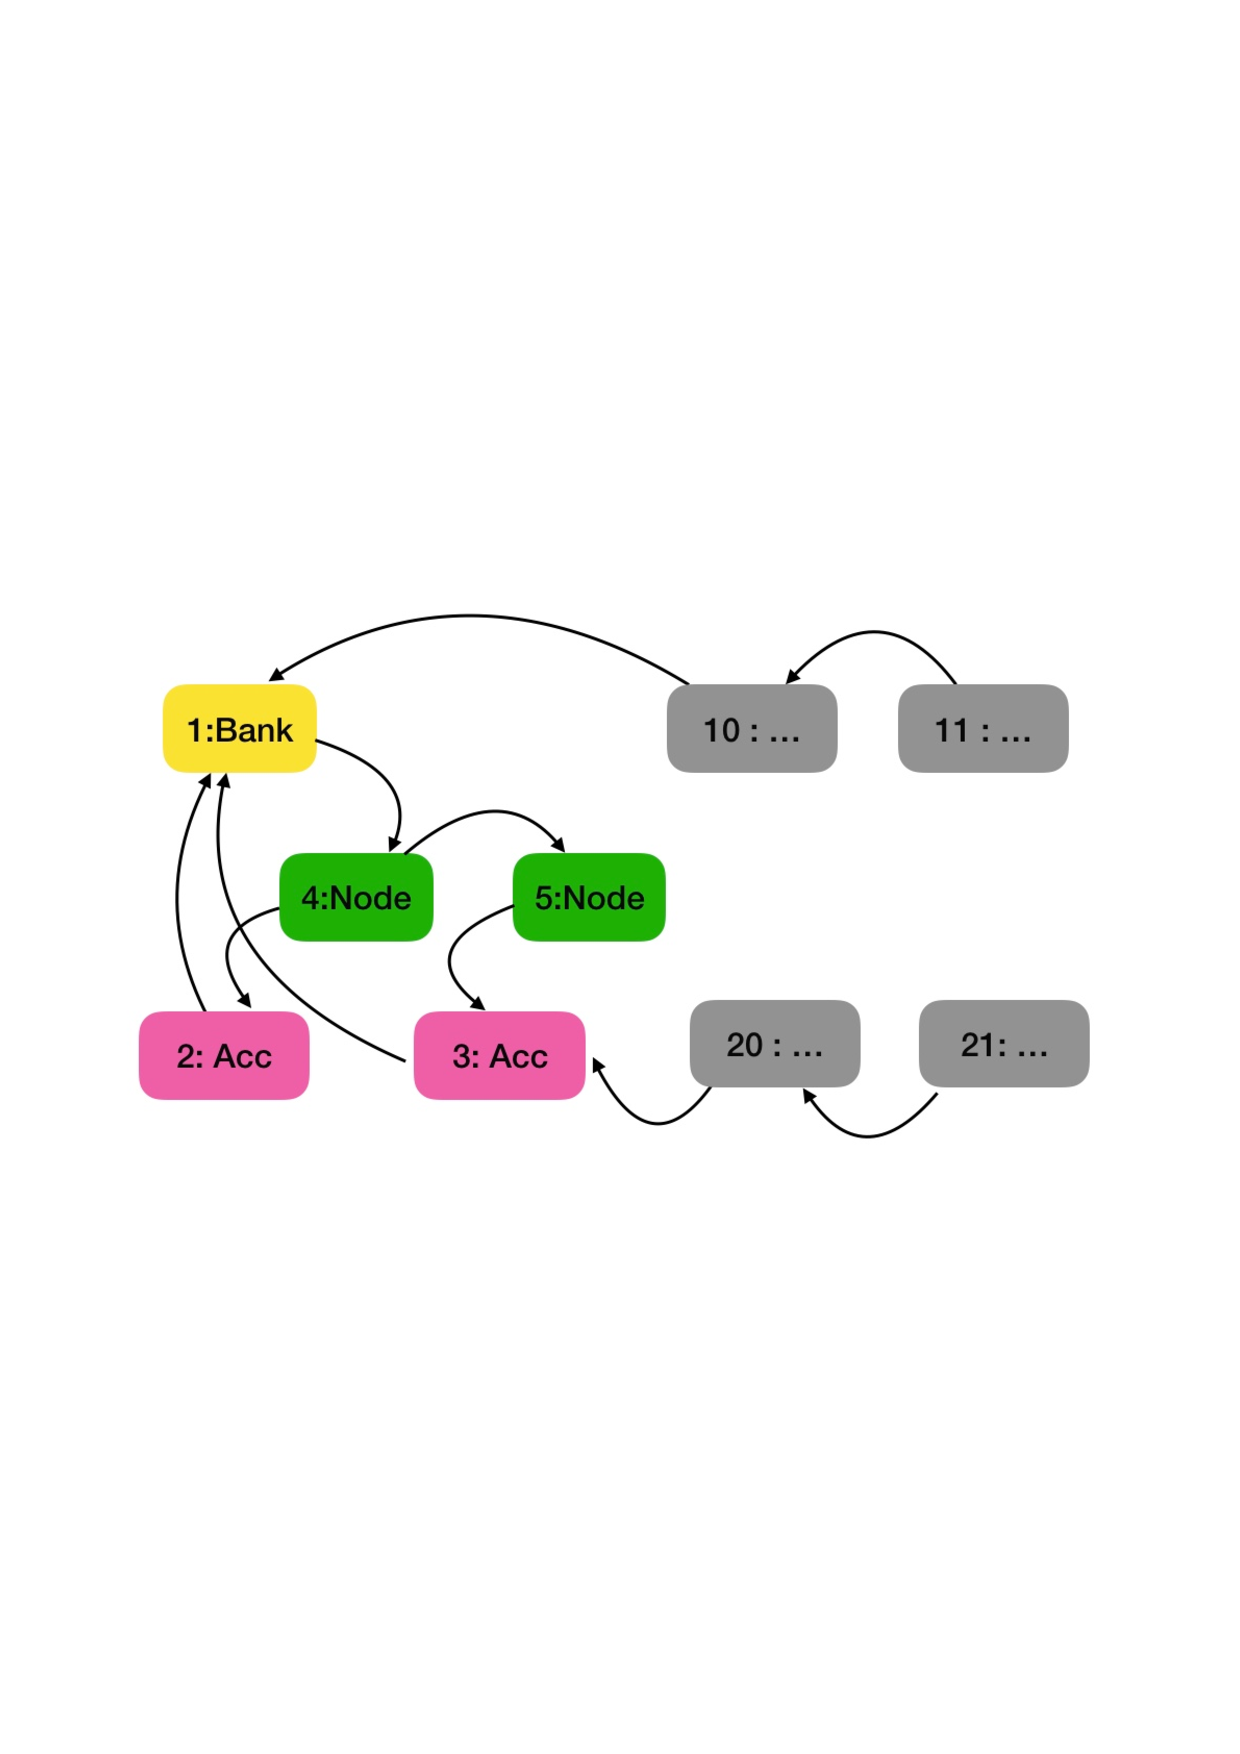
\includegraphics[width=9cm,height=9cm]{diagram}
  %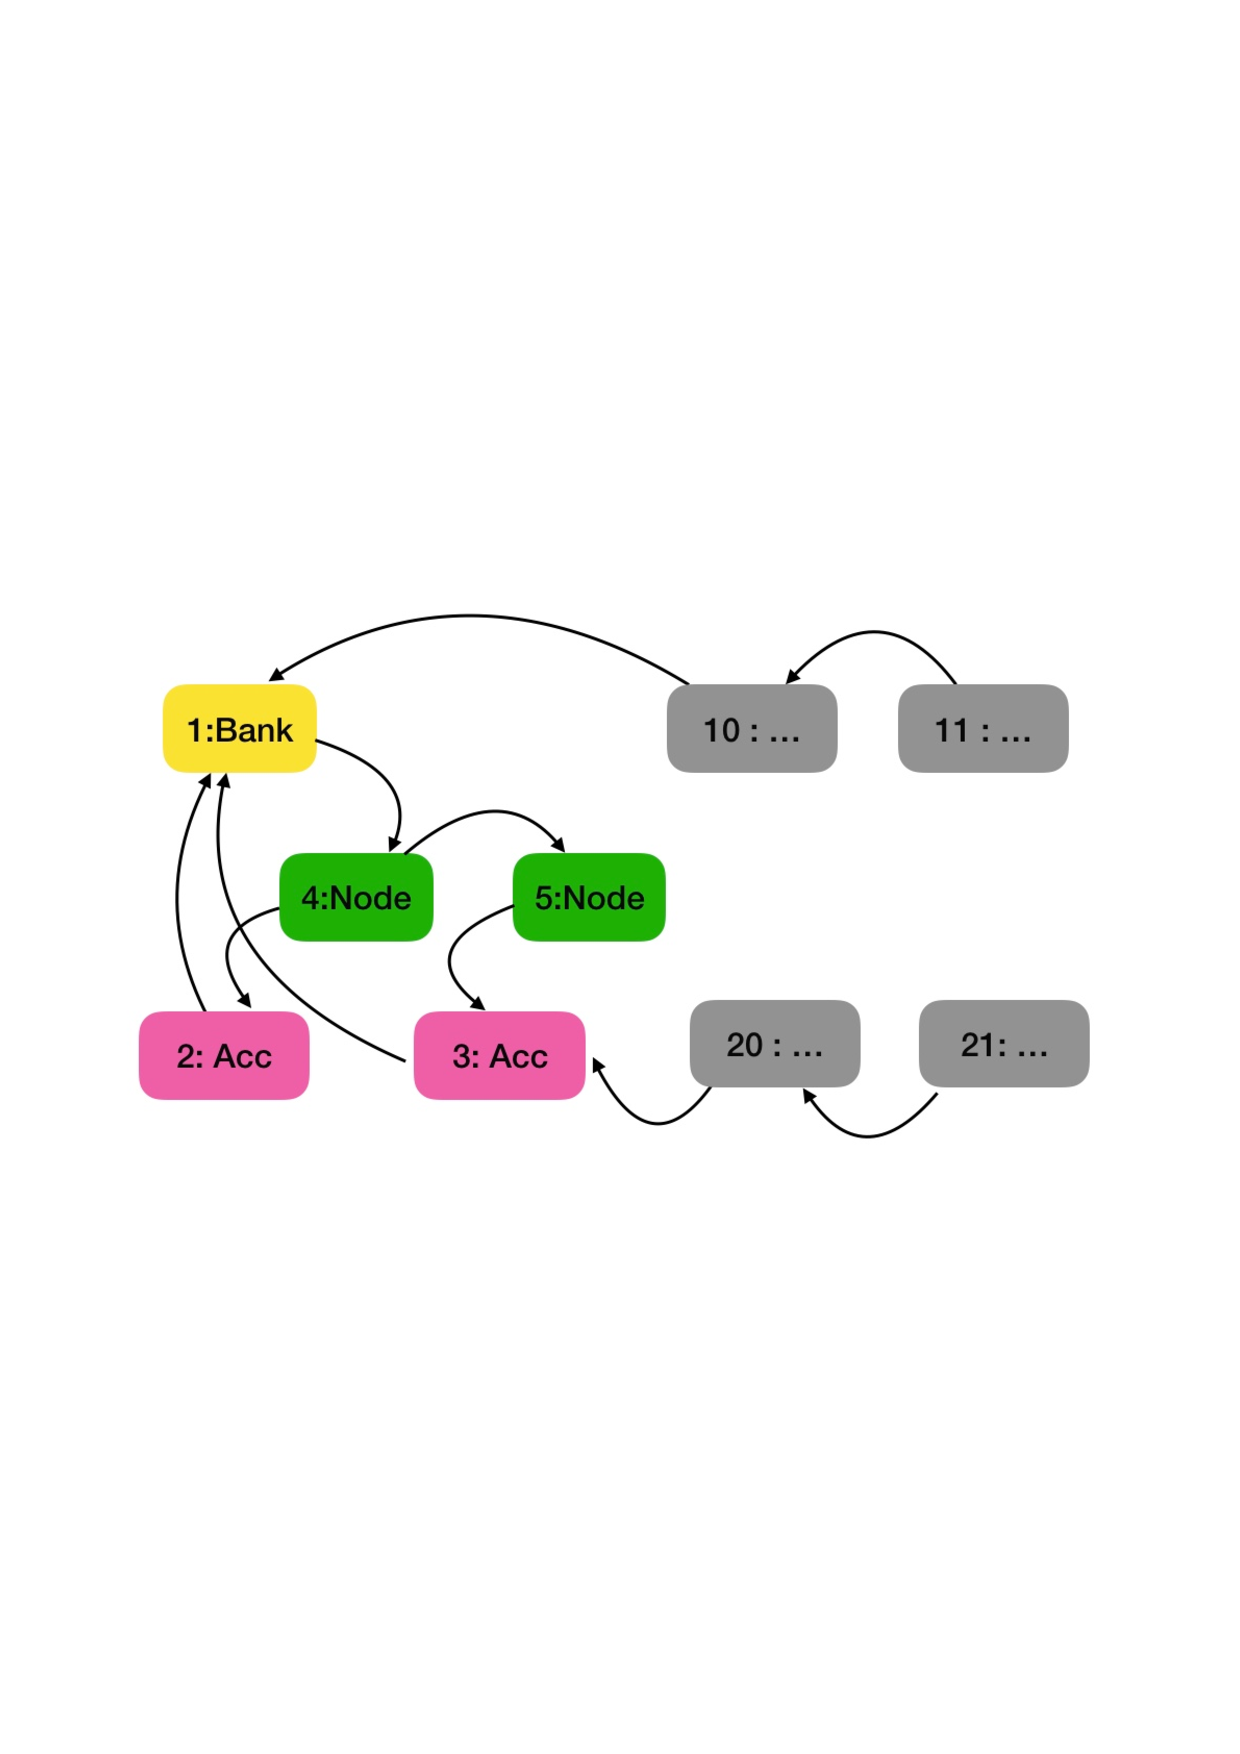
\includegraphics[width=0.5\textwidth]{diagram}
 \caption{Diagrammatic representation of some objects from  \prg{Bank}, \prg{Account} \etc  }
  \label{fig:Diagram}   
  \end{figure}

  
  
 
\section{Permission and Authority}

 
Policy {\bf {Pol\_2}}  ties
{\em authority} with {\em permission}: namely, permission to access the bank is a necessary condition
for authority over the bank's currency.
 %
We will define the OCAP assertions $\CanAccess$  (permission) 
and   $\WillAffect$ (authority). \footnote{Note that they are slightly different 
assertions to those we had in the past.}
Their intuitive meaning is as follows:

\begin{itemize}
\item
% $\M,\sigma  \models \CanAccess(\prg{z},\prg{\sE})$ 
$\CanAccess(\prg{y},\prg{z})$  means that in the current runtime configuration, the object indicated by $\prg{y}$ has {\em direct} access to the object
indicated by  $\prg{z}$. This direct access is given either because $\prg{z}$ is one of \prg{y}'s fields, or because $\prg{z}$
is one of the arguments or local variables in the method body currently executing and that \prg{y} is the receiver.
\item
%$\M,\sigma  \models \WillAffect \lp S, \syntax{\sE}\rp$  
$\WillAffect(\prg{x},\syntax{\sE},\prg{S})$
means the current receiver is \prg{x}, and that 
execution of the current configuration will eventually change the value of $\syntax{\sE}$, and that this execution  
will only involve (ie call methods on, read or write fields from) objects from the set $\prg{S}$.
%\item
%$S \subseteq \prg{C1}\cup \prg{C2} \ldots \cup \prg{Cn}$ expresses that $S$ is a set of objects of runtime class \prg{C1} or \prg{C2} ... or \prg{Cn}.
\end{itemize}

For example, in the runtime configuration from Figure \ref{fig:Diagram}, and assuming that
\prg{x1}, \prg{x10}, \prg{x11} are local variables mapping to addresses \prg{1}, \prg{10}, and \prg{11}, then  we   have that 
$\CanAccess(\prg{x11},\prg{x10})$, and $\CanAccess(\prg{x10},\prg{x1})$, but $\neg \CanAccess(\prg{x11},\prg{x1})$.


The assertion $\WillAffect$  only holds if the set $S$ includes all objects involved in causing the
change of the value of \prg{e}. For example, still in Figure \ref{fig:Diagram}, if the classes of the 
objects at  \prg{x10} and \prg{x11} contain appropriate methods,  and if the current receiver is \prg{11}, then 
it is possible that $\WillAffect(\prg{x11}, \syntax{\prg{x1}.Currency},\{\prg{x11},\prg{x10},\prg{x1}\}, )$,  but regardless of the code in these
objects, we have $\neg \WillAffect(\prg{x11}, \syntax{\prg{x1}.Currency},\{\prg{x11},\prg{x10},\prg{x1}\}, )$


\vspace{.2cm}
 
\noindent
{\em {Definitions and Naming Conventions}} We now proceed with the precise definitions.  Remember first the
naming conventions that  $\M$ stands for a module (ie class definitions), that
$\sigma$ stands for a runtime configuration (ie currently executing sequence of statements with frames and  heap),
  that $\sE$ stands for an expression, that $\interp {\prg{\sE} }{\M,\sigma}$
is the value of the
expression $\sE$ in the state $\sigma$, and  that $\M\vdash \sigma  \leadsto   \sigma'$ expresses that execution of runtime 
configuration $\sigma$   in the context of the class definitions from module $\M$ leads in one small step to $\sigma'$.

\begin{definition}[Permission and Authority ]
\label{def:permission}
Given a module $\M$, identifiers \code{x} and \code{y}, expression $\sE$, and runtime configuration $\sigma$, and a set of addresses $S$, 
we define validity of the assertions $\CanAccess$  and 
$\WillAffect$   as follows:

\begin{itemize}
\item
$\Prog{},\sigma \models   \CanAccess(\prg{x},\prg{y})$   \ iff  \begin{itemize}
\item 
$\sigma(\prg{x},\prg{f})$=$\sigma(\prg{y})$  for some field \prg{f},  or 
\item
$\sigma(\prg{this})$=$\sigma(\prg{x})$ and 
  $\sigma(\prg{z})$=$\sigma(\prg{y})$, 
  $\strut \hspace{0.1cm}$
for some some parameter of local variable \prg{z}.
 \end{itemize}
\item
 $\sigma\mid_S$ denotes a {\em restriction} of $\sigma$ to the objects from the set $S$. That is, the domain of the heap in $\sigma\mid_S$ is $S$, and otherwise,  $\sigma\mid_S$ is identical to $\sigma$.
 \item
$\M,\sigma  \models \WillAffect(\prg{x},S,\syntax{\sE})$  \   iff  
\begin{itemize}
\item $\sigma(\prg{this})$=$\sigma(\prg{x})$ and
\item  $\exists \sigma'.$ 
  $ \M\vdash \sigma\mid_S  \leadsto^*   \sigma'$, and   $\interp {\syntax{\sE}} {\M,\sigma} \neq  \interp {\syntax{{\sE}}} {\M,\sigma'}    $.
\end{itemize}
\item
$\M,\sigma  \models \WillAccessThrough(\prg{x},S,\prg{y})$  \   iff  
\begin{itemize}
\item  $\exists \sigma'.$ 
  $ \M\vdash \sigma\mid_S  \leadsto^*   \sigma'$, and   $\M, \sigma' \vdash \CanAccess(\prg{x},\prg{y})$.
\end{itemize}


\end{itemize}
\end{definition}

We can easily prove the following lemma:

\begin{lemma}
For   sets $\prg{S}$ and  $\prg{S}'$, runtime configuration $\sigma$, variable $\prg{x}$ and expression $\prg{e}$, if
$\sigma \models \prg{S} \subseteq \prg{S}'$, then
\begin{itemize}
\item
$\sigma \models \WillAffect(\prg{x},\syntax{\sE},\prg{S})$\  implies\ 
$\sigma \models \WillAffect(\prg{x},\syntax{\sE},\prg{S}')$.
\item
$\sigma \models \WillAccessThrough(\prg{x},\prg{y},\prg{S})$\  implies\ 
$\sigma \models \WillAccessThrough(\prg{x},\prg{y},\prg{S}')$.

\end{itemize}
\end{lemma}



  
\section{Invariants}

% The policy  \code{Pol\_protect\_currency} in figure \ref{fig:ValidBank} is an invariant.
% A policy is an invariant if it has to hold in any state reachable
% from execution in the code of $\M$ linked together with any other code.
We define below the meaning of invariants.\footnote{This part is as we had defined previously, with two simplifications: a) we do not need to worry about the $\obeys$-predicate here, and b) we do not distinguish the names of the classes and the names of participants in interfaces.}
The assertion $\M   \models\  \A$ requires that  the assertion $A$ is satisfied 
in all reachable states.
The   set  $\Arising(\M)$ contains all runtime configurations which can be reached
when starting with an empty heap,  and executing any expression consisting of constructor  and method calls
as defined in $\M$.\footnote{That is,
$\Arising(\M)$=$\{ \ \sigma\ \mid\ \exists \prg{e}.\ \M \vdash (\prg{e},\emptyset) \leadsto* \sigma \ \}$}
The term 
%$\prg{x}:\prg{C}$ expresses that $\interp {\prg{x} }{\M,\sigma}$ is the address of an object of class \prg{C};
$\M*\M'$ denotes the result of linking two modules -- the operation is defined only when the
two modules do not have overlapping definitions.


 
  

\begin{definition}[Invariants]
\label{def:invariant}
\noindent
For a module $\M$  and assertion $\A$ we define:\\

 \begin{itemize}
 \item
$\M   \models\  \A$\ \ \  iff\ \ \ \ 
% $\strut\SP\SP$
$\forall \M'.\, \forall \sigma\!\in\!\Arising(\M'*\M).\ \M'*\M,\sigma \models \  \A$
 \end{itemize}
\end{definition}

The use of the set of configurations from $\Arising(\M'*\M)$ reflects that policies
 need to hold in an {\em open} world, where
we link against {\em any} module $\M'$, 
about which we know nothing. 
% 
% which does not necessarily use the objects created in $\M$
%in the way these objects have been specified.
%Thus, the policy $A$ has to hold in an   {\em open} system:  it has to hold in the presence of {\em any} other code.
%In particular, class \prg{C}  may not make any assumptions about the order nor the states from
%  which its methods/constructors are called from the code in $\M'$ called\footnote{Its public methods may not have any preconditions}, other
%than those it can establish  and maintain itself, and can confidently know  are not broken by the
%code in $\M'$. This means that the code of \prg{C} needs to protect
%sensitive data, and expose only the functionality which will preserve $A$.
%The protection may be afforded in many different ways: through objects which
%attenuate authority, through cryptography, or through language mechanisms such
%as private methods, constant fields\cite{immut}, or owned data \cite{ClaPotNobOOPSLA98}.
% This leads to defensive, robust programming.\footnote{Here again, the full definition has the form $\M   \modelsWithO\  \prg{C}\, :\,\A$}.
 
 \section{Specifying  {\bf {Pol\_2}} and  {\bf {Pol\_4}}}

We    give a formal definition of {\bf {Pol\_2}} and  {\bf {Pol\_4}}, using the concepts defined earlier in  Definition \ref{def:permission}: %

\begin{definition}
\label{def:pol2}
We define   {\bf {Pol\_2}}  and   {\bf {Pol\_4}} as follows:

%  \noindent
  {\bf {Pol\_2}}\ \  $\equiv$\ \ $\forall \prg{b}.\forall \prg{o}.\forall \prg{S}.\ [ \ \  \ \ \prg{b}:\prg{Bank}\ \wedge\  \prg{b}\neq \prg{o}\ \wedge \ \WillAffect(\prg{o},\prg{b.Currency},\prg{S})  $\\
  $\strut \hspace{4cm}  \longrightarrow$\\
 $\strut \hspace{3.9cm}  \exists \prg{o}'.\ [\, \prg{o}'\in \prg{S}\ \wedge \  \CanAccess( \prg{o}', \prg{b} )\ \wedge\ \neg (\, \prg{o}' : \prg{Account} \, ) \ ] \  \  \ \  ]$
 
 \vspace{.1cm}
% \noindent
    {\bf {Pol\_4}}\ \  $\equiv$\ \ $\forall \prg{a}.\forall \prg{o}.\forall \prg{S}.\ [ \ \  \ \  \prg{a}:\prg{Account} \wedge \prg{a}\neq\prg{o} \wedge \WillAffect(\prg{o},\prg{a.Balance},\prg{S}) $\  \\
  $\strut \hspace{4cm}  \longrightarrow$ \\
 $\strut \hspace{3.9cm} \exists \prg{o}'.\ [\, \prg{o}'\in \prg{S}\ \wedge \ \CanAccess( \prg{o}', \prg{a} )\ \wedge \neg (\  \prg{o}' : \prg{Account}\ \cup\ \prg{Bank}\, ) \ ] \ \ \ \ ]$

\end{definition}


{\bf {Pol\_2}}  guarantees
that if an object \prg{o}$\neq$\prg{b} may affect the value of \prg{b.Currency} only if the  objects 
involved in the process of affecting the value of \prg{b.Currency}  include at least an object $\prg{o}'$ 
which had direct access to \prg{b}, and 
whose class is  not  \prg{Account}. Stated positively, this policy mandates 
that exporting an \prg{Account} to an environment will not affect the \prg{Currency} of \prg{b}.  
In other words,
\prg{Account}s protect the integrity of the \prg{Bank}'s currency.
 
 
In more detail, by applying  Definition \ref{def:invariant} on Definition \ref{def:pol2}, the  meaning of policy {\bf {Pol\_2}}  
  is, that a runtime configuration $\sigma$ satisfies  {\bf {Pol\_2}}  if whenever the current receiver in $\sigma$
 is not a \prg{Bank} object, and the execution of $\sigma$ leads to another runtime configuration $\sigma'$ 
 with a different value for \prg{b.Currency}, then the objects involved in the execution from
 $\sigma$ to $\sigma'$ include at least one object which had direct access to \prg{b}. 
 Note that this direct access needs to exist at the beginning of   the execution, \ie at $\sigma$.
 Formally:
 
 \noindent
 $\M, \sigma \models   {\bf {Pol\_2}}$\\$ \strut \ \ \ \  \ \  \longleftrightarrow $\\
 $\forall \prg{b}.\forall \prg{o}.\forall \prg{S}.\ [ \ \ \ \ \M, \sigma \models \prg{b}:\prg{Bank}\ \wedge\  
 \sigma(\prg{b})\neq \sigma(\prg{o})\ \wedge \ 
 \sigma(\prg{this}) = \sigma(\prg{o}) $\\
 $\strut \hspace{2.1cm}  \wedge \
 \ \exists\sigma'.(\ \ \ \ \M \vdash \sigma\mid_{\prg{S}}  \leadsto^* \sigma'\
\ \wedge\ \interp {\prg{b.Currency}}{\M,\sigma}\neq \interp {\prg{b.Currency}}{\M,\sigma'}\ )$\\
$\strut \hspace{4.7cm} \longrightarrow$ \\
 $\strut \hspace{2.1cm}  \exists \prg{o}'. (\ \  \sigma(\prg{o}')
\!\!\in\!\!\prg{S}\ \wedge \ \M, \sigma \models \CanAccess( \prg{o}', \prg{a} )\ \wedge \  \ClassOf{\prg{o}'}{\sigma}\!\!\notin\!\!\{ \prg{Account}, \prg{Bank}\}    \ )  \ \ \ \  ]$
 
\vspace{.1in}  
And by applying the Definition 1, again, we obtain that a module $\M$ satisfies {\bf {Pol\_2}}, if any configuration $\sigma$ which arises 
from the combination of $\M$ with any other module $\M$, also satisfies {\bf {Pol\_2}}. Formally:

\noindent
$\M  \models   {\bf {Pol\_2}}$\\$ \strut \ \ \ \  \ \  \longleftrightarrow $\\
 $  \forall \M'. \forall \sigma\!\in\!\Arising(\M'*\M).\ \M'*\M,\sigma \models  {\bf {Pol\_2}}$
 
 
%In Figure \ref{fig:Pol2} we show the  meaning of policy {\bf {Pol\_2}} in more detail, by applying  Definition 1:
%That is, a runtime configuration $\sigma$ satisfies  {\bf {Pol\_2}}  if whenever the current receiver in $\sigma$
%is not a \prg{Bank} object, and the execution of $\sigma$ leads to another runtime configuration $\sigma'$ 
%with a different value for \prg{b.Currency}, then the objects involved in the execution from
%$\sigma$ to $\sigma'$ include at least one object which had direct access to \prg{b}. 
%Note that this direct access needs to exist at the beginning of   the execution, \ie at $\sigma$.

\section{Reasoning about encapsulation}

It is natural in programming to require that certain values do not "leak" out of data structures. For example,
a \prg{Account} does not leak an other \prg{Account} or a \prg{Node} or a \prg{Bank}. 
\footnote{Such policies have not been required as such in \cite{Elang}, but are useful in reasoning about programs. TODO: Strengthen this discussion}.
Using the predicate $\WIlAccessThrough$ we can specify that values are encapsulated.

We define a further policy 

\begin{description}
\item[Pol\_7]
The \prg{Bank} does not leak out of the \prg{Bank}/\prg{Account} system
\end{description}

And we give a formal specification

\begin{definition}[Banks do not leak]
\label{def:bankNoLEak} We define {\bf {Pol\_7}} as follows:

{\bf {Pol\_7}}\ \  $\equiv$\ \ $\forall \prg{b}.\forall \prg{o}.\forall \prg{S}.\ [ \ \  \ \ \prg{b}:\prg{Bank}\ \wedge\  \neg (\, \prg{o}' : \prg{Account} \, )  \wedge \ \prg{b}\neq \prg{o}\ \wedge \ \WillAccessThrough(\prg{o},\prg{b},\prg{S})  $\\
  $\strut \hspace{4cm}  \longrightarrow$\\
 $\strut \hspace{3.9cm}  \exists \prg{o}'.\ [\, \prg{o}'\in \prg{S}\ \wedge \  \CanAccess( \prg{o}', \prg{b} )\ \wedge\ \neg (\, \prg{o}' : \prg{Account} \, ) \ ] \  \  \ \  ]$

\end{definition}



\section*{Bibliography} 
  % \bibliographystyle{plain}
 \bibliography{Case}



\end{document}

